\section{Effets des vents}

\subsection{Modèle linéaire, phénomènes dissipatifs et filtre atmosphérique}

Les IGW représentent une solution des équations primitives atmosphériques (équation de Navier-Stokes \ie de la quantité de mouvement $\rho \vv$ pour un fluide newtonien) associées à des équations de conservation et/ou d'état bien choisies. Dans un modèle d'atmosphère réaliste, la masse volumique $\rho$ ne peut pas être considérée comme constante. Outre le champ de vitesse 3D $\vv$ et $\rho$, la pression $P$ apparaît évidemment comme cinquième inconnue. \cite{Occhipinti2008} proposent un système fermé basé sur les équations de continuité et de non-divergence, en l'absence de forçage :
\begin{subnumcases}{\label{eq:systeme}}
    \lp \delt{} + \vv \cdot \gradient \rp \vv &    $= -\frac{1}{\rho} \gradient P$    \label{eq:systeme-un} \\
    \divergence \vv &                      $= 0$                                                \label{eq:systeme-deux} \\
    \delt \rho + \divergence{\rho \vv} &   $= 0$                                                \label{eq:systeme-trois}
\end{subnumcases}

Ce modèle permet une étude directe de l'effet des vents. L'équation \refeq{eq:systeme-un} contient un terme advectif dont la complexité peut être réduite en considérant une approximation linéaire. Les ondes sont décrites comme la manifestation d'un (petit) écart à un état d'équilibre, dont la seule dépendance sera ici en $\textbf z$. On décompose ainsi $X \in \{ \vv = (u, v, w), \rho, \pression \}$ en la somme d'une partie moyenne $X_0(z)$ et d'une perturbation $X_1(x,y,z,t)$ (très petite devant la partie moyenne). Par ailleurs, sur la base d'une analyse en ordre de grandeur, on décide de négliger $\uzc$ devant $\uxc$ et $\uyc$. On applique l'approximation de Boussinesq (\ie $\rho_0$ partout sauf sur le terme de flottabilité, affecté de la perturbation — cela implique la non-divergence de la vitesse totale). Enfin, on linéarise au premier ordre en effectuant des développements limités sur $\rho$ au premier ordre (simplifiant les termes de pression et de gravité) et en ne prenant pas en compte les termes quadratiques et supérieurs ni les produits de perturbations. On cherche alors la solution de l'équation d'onde pour les cinq inconnues,  en prenant les transformées en ondes planes $X_1(x,y,z,t) = \tilde X(z) \cdot {\mathrm e^{i(\overbrace{k_x x + k_y y - \omega t}^{\textrm{phase~} \Phi})}}$. On obtient alors le système suivant dans le domaine spectral :
\begin{subnumcases}{\label{sys:S}(S)}
i \Omega \tux - \tuz \dz \uxc - \frac{1}{\rho_0} i k_x \tp = 0             \label{eq:igw-un}        \\
i \Omega \tuy - \tuz \dz \uyc - \frac{1}{\rho_0} i k_y \tp = 0             \label{eq:igw-deux}      \\
i \Omega \tuz - \frac{1}{\rho_0} \dz \tp - \frac{\trho}{\rho_0} g = 0      \label{eq:igw-trois}     \\
i k_x \tux + i k_y \tuy + \dz \tuz = 0                                     \label{eq:igw-quatre}    \\
i \Omega - \tuz \dz{\rho_0} = 0                                            \label{eq:igw-cinq}
\end{subnumcases}
avec $\Omega = \omega - \uxc k_x - \uyc k_y$ la fréquence intrinsèque liée au repère en mouvement.

Le fait de conserver des dérivées en $z$ en utilisant une phase spatialement 2D permet d'exprimer S sous la forme d'un propagateur du type $\dz V = A V$, avec :
\begin{align}
V & =
\begin{pmatrix}
    \tuz^* \\
    \tp^*
\end{pmatrix} \\
A & =
\begin{bmatrix}
    -\frac{1}{\Omega} \lp k_x \dz \uxc + k_y \dz \uyc \rp + \frac{1}{2} \dz{\ln{\rho_0}} & -\frac{i \lp k_x^2 + k_y^2 \rp}{\Omega}   \\
    i \lp \Omega + \frac{g}{\Omega} \dz{\ln{\rho_0}} \rp                                  & -\frac{1}{2} \dz{\ln{\rho_0}}             \notag
\end{bmatrix}
\end{align}
Les $*$ dénotent une renormalisation des deux paramètres $\tuz$ et $\tp$ : $\tuz^* = \sqrt{\rho_0} \tuz$ et $\tp^* = \frac{\tp}{\sqrt{\rho_0}}$ (d'où les termes en $\pm \frac{1}{2} \dz{\ln{\rho_0}}$). Cette renormalisation proportionnelle à la racine carrée de l'énergie assure que les perturbations de la vitesse verticale et de la pression sont indépendantes de l'amplification exponentielle avec $z$. Au final, le système ainsi construit permet une étude modale atemporelle pour ces deux inconnues, en fonction de l'état moyen de l'atmosphère (profils des vents, de densité, …) et du choix des paramètres spectraux, \ie périodes et longueurs d'onde.

Dans ces équations n'apparaissent pas explicitement de termes dissipatifs, lesquels seraient liés par exemple à de la dissipation thermique, des interactions d'ondes, du déferlement, ou bien de la diffusion de quantité de mouvement (viscosité). La théorie linéaire dérivée dans ces conditions se prête bien à une étude modale mono-paramétrique, mais il faut garder à l'esprit que les ordres de grandeur absolus déduits de simulations opérées sous ces conditions n'ont qu'une valeur limitée, car les mécanismes dissipatifs et les interactions multi-échelles sont vraisemblablement primordiaux dans les cas réalistes (\cite{Fritts2003}). Par ailleurs, en ne considérant ni les transferts au flux moyen, ni la turbulence induite, ni les échanges de chaleur, on ne s'autorise aucun \emph{feedback} lors de la propagation pseudo-spectrale. C'est donc avec un modèle « découplé » que le travail numérique a été effectué.

% copcol depuis l'autre .tex le système linéarisé, sans viscosité, le propagateur.
% parler des phénomènes dissipatifs en général, puis des deux paramètres étudiés : vent et viscosité
% pour le vent, en fait c'est pas toujours dissipatif ! étude de Sun et al, puis mon objectif : vérifier et étudier un cas « réaliste » d'un point de vue modal (filtre directionnel)

% nouvelle partie, sur les vents :
% dire comment on le passe en numérique, que j'ai fait une version vectorielle assez stable et rapide
% décrire les deux types d'instabilité : limite acoustique, ok, et explosion, qui elle fait référence à la partie suivante (préconditionnement)
% code en annexe, clean, décrire vite fait son fonctionnement
% donner des résultats parlant : un truc paramétrique, et un pour le modèle

Un double objectif a été poursuivi dans la paramétrisation par les vents moyens :
\begin{itemize}
    \item vérifier avec un modèle mono-paramétrique les résulats de \cite{Sun2007} qui, sur la base d'une analyse spectrale, estiment que les vents pourraient agir comme un filtre directionnel, permettant aux IGW se propageant contre le vent moyen d'atteindre plus rapidement et avec un minimum de perte énergétique la ionosphère ;
    \item examiner le rôle des vents moyens issus d'un modèle réaliste.
\end{itemize}

\subsection{Implémentation numérique}

En relation avec \cite{Occhipinti2008} existait un code de test MATLAB itératif, pour lequel les dimensions horizontales étaient réduites à une seule. Il servait à valider des calculs en amont d'une implémentation dans un code FORTRAN 3D entièrement spectral destiné à traiter des jeux de données massifs sur des architectures puissantes. L'étude de l'effet des vents à été menée sur la base du code MATLAB, transformé en un solveur vectoriel (\hyperref{annexe:A:modesTvectwind.m}{}{}{modesT-vect-wind.m}).

Le propagateur décrit ci-avant a été discrétisé par des différences finies centrées afin de fournir un système linéaire du type $KU~=~B$, avec $U$ le vecteur solution (contenant autant de couples $\lp \tuz^*~~\tp^* \rp$ que de pas de calculs), $B$ le vecteur second membre (identiquement nul, sauf pour les conditions initiales) et $K$ une matrice creuse de cœfficients issus du propagateur. Le couple de conditions initiales traduit la continuité de la perturbation de la vitesse verticale au sol (premier pas d'intégration), qui a été prise unitaire dans la perspective d'une étude modale prénormalisée. La pression initiale est déduite des caractéristiques spectrales imposées pour l'étude ($P_0 \propto (\omega, k_x, k_y, k_z)$ et $k_z \propto (k_x, k_y, N^2)$ où $N^2$ est la fréquence de Brunt–Väisälä).

En plus de la version vectorielle pseudo-3D (ondes sphériques), des scripts annexes (\hyperref{annexe:A:windeffect.m}{}{}{wind-effect.m}, \hyperref{annexe:A:dataprocessing.m}{}{}{data-processing.m}, \hyperref{annexe:A:mantexpnt.m}{}{}{mantexpnt.m}) ont été développés pour traiter les données (extraction, détection de la divergence, etc.) et produire des sorties graphiques synthétiques.

% TODO
% Le modèle d'atmosphère utilisé
% le modèle de vents
% dire que le code itératif avait deux types de divergence (acoustique, précision) et que le domaine de stabilité a été étendue pour la seconde avec le code vectoriel

\subsection{Résultats}

L'étude spectrale de \cite{Sun2007} repose également sur la théorie linéaire des IGW dans l'approximation des petites perturbations. Une fonction de transfert proche du propagateur présenté ci-avant est utilisée pour explorer les caractéristiques de la propagation atmosphérique, dans un modèle avec une composante visqueuse et des transferts de chaleur. De façon analogue, l'interface sol--atmosphère porte le signal d'entrée et les conditions initiales. Il est montré que, pour un modèle de vent moyen SE-NW (HWM93, \cite{Hedin1991}), les IGW dans la bande de période de 15 à 30 mn et de longueur d'onde de 200 à 400 km ont le plus de chance d'atteindre 300 km d'altitude, surtout si elles se propagent contre le vent moyen (\ie dans une direction NE-SW).

Les tsunamis sont associés à des périodes de l'ordre de quelques minutes à une heure, avec des longueurs d'ondes de 10 à 500 kilomètres. Compte tenu de la relation donnant la vitesse des ondes surfaciques induites, pour une hauteur moyenne océanique de 2500 km, on trouve que le domaine spectral dans lequel se réalise en première approximation le transfert d'énergie entre les ondes tsunamigéniques et les IGW correspond assez bien au domaine mis en évidence par Sun \emph{et al.} Toutefois, une large gamme de couples fréquence/nombre d'onde sont envisageables en raison des sources multiples d'IGW.

La figure \ref{fig:modes-scales} présente les résultats d'une simulation 2D sur trois fréquences, pour des IGW portant les caractéristiques spectrales d'une source tsunamigénique, associées à un gradient de vent linéaire fixé de 0 à $\pm$ 20 m.s$^{-1}$, et pour une gamme de trois longueurs d'onde initiales imposées par la relation entre nombre d'onde, période et vitesse de phase. On observe une augmentation de l'amplitude de la perturbation de la vitesse verticale avec un écrasement des modes, bien marqués après 125 km. Cette altitude correspond à la thermopause, à partir de laquelle a lieu un transfert énergétique entre les champs de pression, de densité et de vitesse horizontale d'une part, et le champ de vitesse verticale d'autre part. La thermosphère ainsi perturbée, et plus particulièrement la ionosphère, peut jouer le rôle d'amplificateur, un processus auquel se surimposera l'effet des vents. 

Le même type de simulation à basse résolution a été réalisé avec un modèle de vent NRLMSISE-00 (\cite{Picone2002}, figure \ref{fig:nrlmsise}). On observe (figure \ref{fig:modes-scales-picone}) une modulation des modes (en terme de valeur des maximums normalisés d'amplitude de la perturbation de vitesse verticale) en fonction du régime des vents moyens. Une comparaison des simulations avec vent zonal seul, vent méridional seul et le couple de vents montrerait que la composante de vent perpendiculaire à la direction de propagation des IGW n'a que peu d'influence sur celle-ci. Les vents contraires ont en effet tendance à écraser le paquet d'onde, et les vents portant à l'étaler, ce qui conduit respectivement à une diminution et une augmentation de la dissipation énergétique lors de la propagation, avec une dépendance à l'angle entre direction de propagation et direction du vent moyen. En l'absence de termes dissipatifs associés à la diffusion moléculaire et thermique, les variations d'amplitudes maximales affectent des gammes de périodes un peu plus élevées que pour Sun \emph{et al.}, mais l'observation principale est que l'intensité du gradient de vent est le facteur principal pour l'amplification dans le modèle mono-paramétrique, avant les caractéristiques fréquentielles de l'IGW soumise à ce gradient. Dans un cas réaliste, les phénomènes dissipatifs, outre leur effet additionnel de filtre spectral, entraveront l'amplification.

\begin{figure}[!ht]
\centering
\subfigure[]{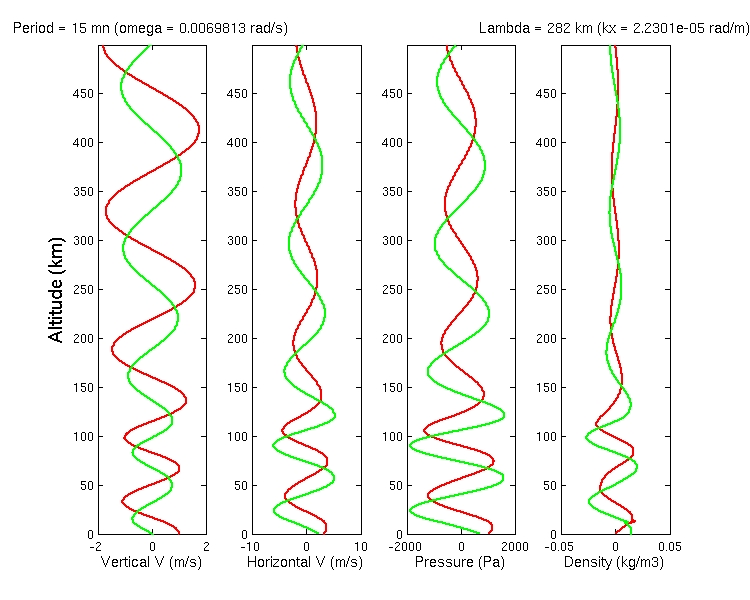
\includegraphics[width=0.45\linewidth]{01}}
\subfigure[]{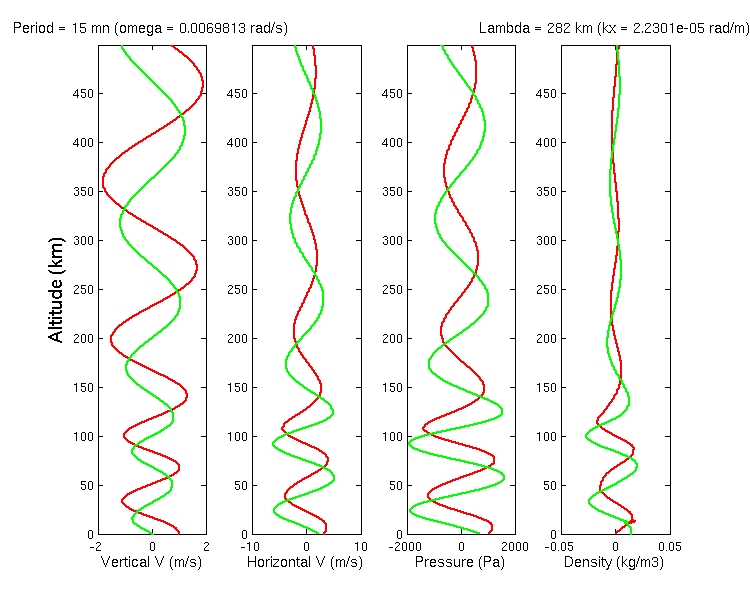
\includegraphics[width=0.45\linewidth]{03}}\\
\subfigure[]{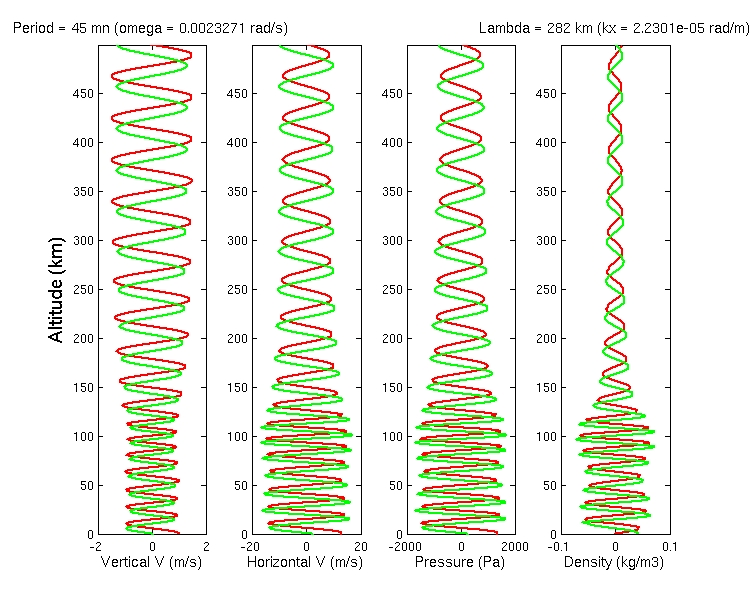
\includegraphics[width=0.45\linewidth]{02}}
\subfigure[]{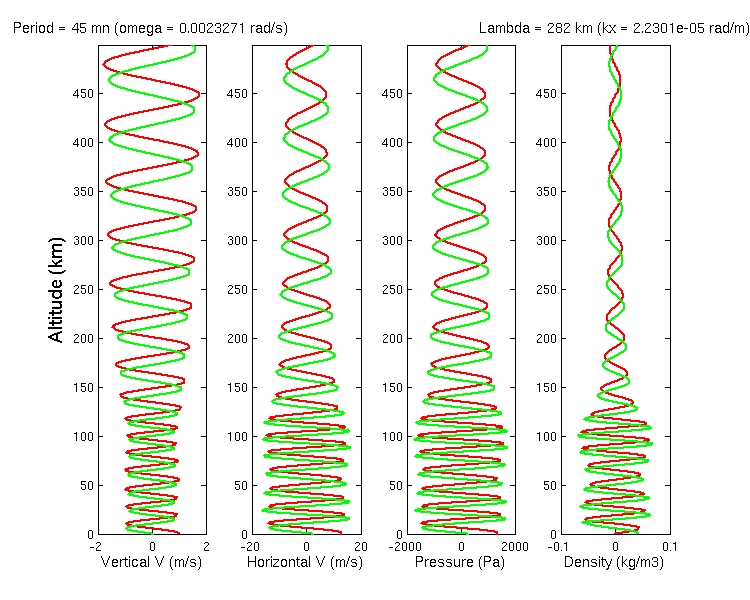
\includegraphics[width=0.45\linewidth]{04}}\\
\subfigure[]{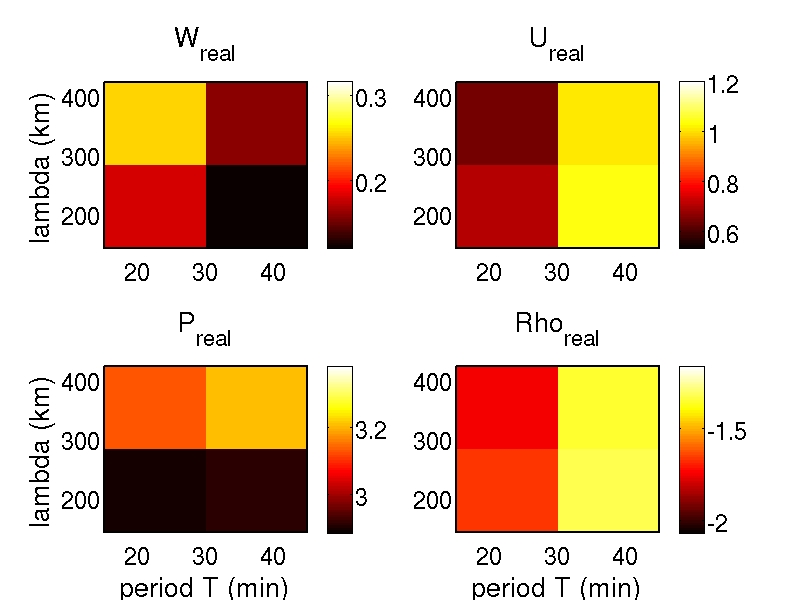
\includegraphics[width=0.45\linewidth]{05}}
\subfigure[]{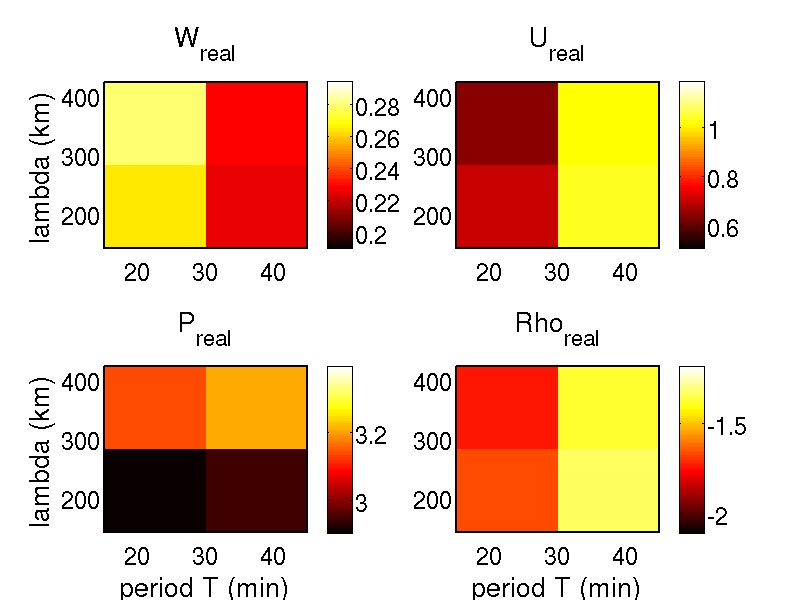
\includegraphics[width=0.45\linewidth]{06}}
\caption{Modes reliés à une onde tsunamigénique pour un gradient de vent linéaire de 0 à 20 m.s$^{-1}$ (a, c, e) et de 0 à -20 m.s$^{-1}$ (b, d, f). Périodes de 15 mn (a, b) et 45 mn (c, d). Maximum d'amplitudes respectifs dans l'espace des $k-\lambda$ (e, f).}
\label{fig:modes-scales}
\end{figure}

\clearpage
\changepage{3cm}%amount added to textheight
           {}%amount added to textwidth
           {}%amount added to evensidemargin
           {}%amount added to oddsidemargin
           {}%amount added to columnsep
           {-2cm}%amount added to topmargin
           {}%amount added to headheight
           {}%amount added to headsep
           {}%amount added to footskip
\begin{figure}[!ht]
\centering
\subfigure[]{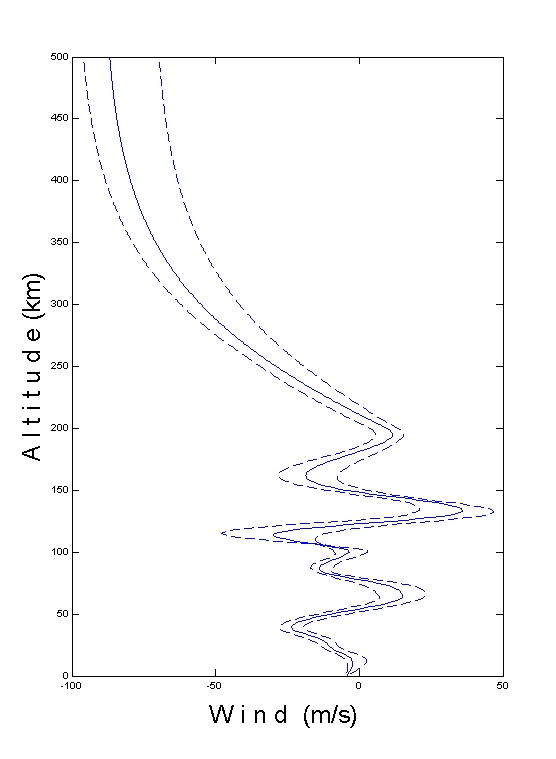
\includegraphics[width=0.3\linewidth]{Wind_Z}}
\subfigure[]{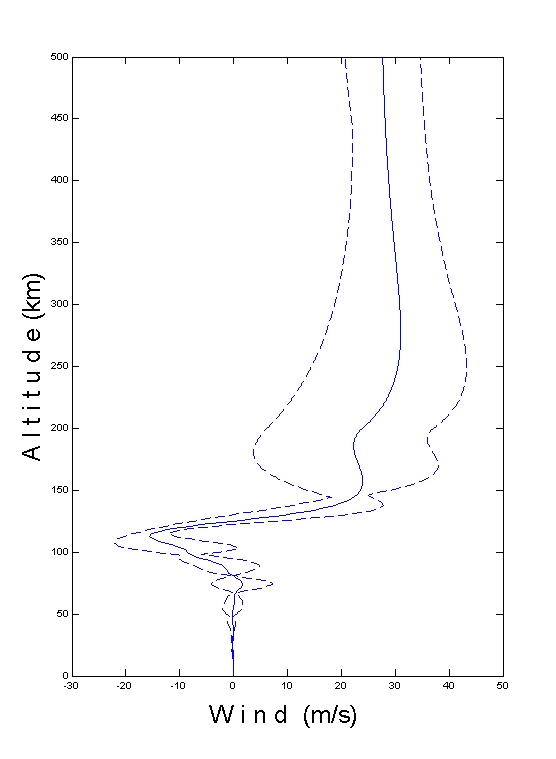
\includegraphics[width=0.3\linewidth]{Wind_M}}\\
\caption{Modèle de vent NRLMSISE-00 à 01H00 UT. Vent zonal (a) et vent méridien (b). Les courbes pleines sont les profils aux coordonnées géographiques [0°N; 85°E] (utilisés pour les simulations numériques), les lignes en pointillés montrent les variations des valeurs dans une grille de coordonnées [$\pm$12°N; (75°E,95°E)].
}
\label{fig:nrlmsise}
\end{figure}

\begin{figure}[!ht]
\centering
\subfigure[]{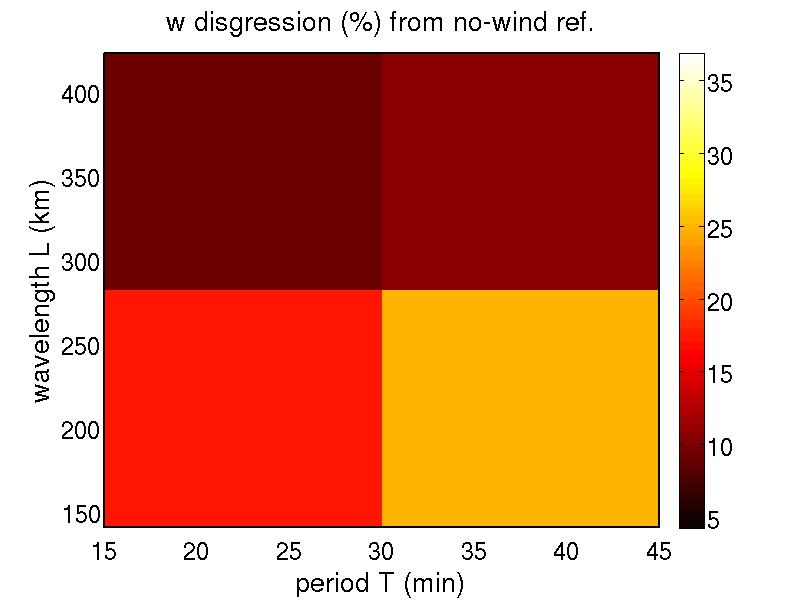
\includegraphics[width=0.4\linewidth]{disgression-w0-20T15+30+45Lauto}}
\subfigure[]{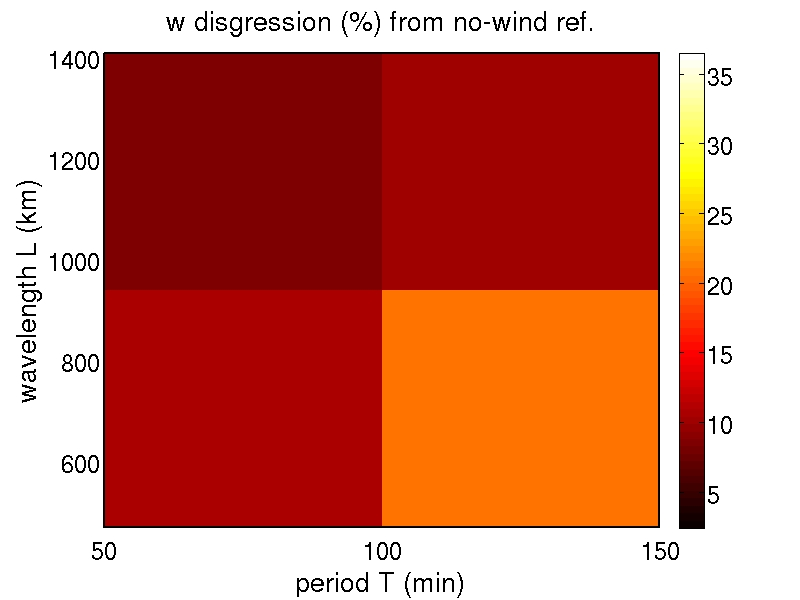
\includegraphics[width=0.4\linewidth]{disgression-w0-20T50+100+150Lauto}}\\
\subfigure[]{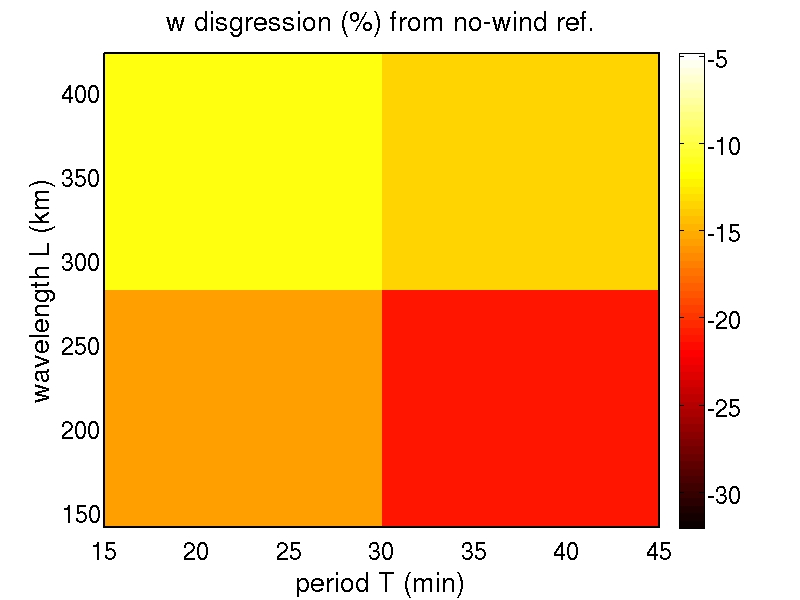
\includegraphics[width=0.4\linewidth]{disgression-w0+20T15+30+45Lauto}}
\subfigure[]{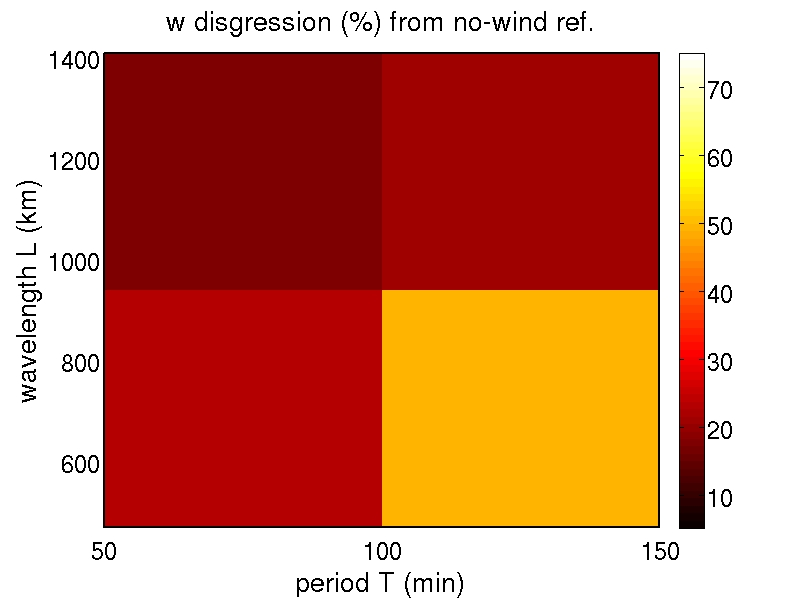
\includegraphics[width=0.4\linewidth]{disgression-w0-50T50+100+150Lauto}}
\caption{Écarts entre les maximums d'amplitude normalisés dans une atmosphère neutre pourvue d'un profil de vents moyens NRLMSISE-00 et les maximums normalisés pour une atmosphère neutre sans vents : pour un gradient de vent de 0 à -20 m.s$^{-1}$ pour deux gammes de fréquences (a, b), pour un gradient de vent de de 0 à +20 m.s$^{-1}$ (c), pour un gradient de vent de 0 à -50 m.s$^{-1}$ (d).}
\label{fig:modes-scales-picone}
\end{figure}
\vfill
